\chapter{Validação da Arquitetura}

Um dos objetivos desta dissertação passa por demonstrar a capacidade da arquitetura implementada em recolher e processar informação através da utilização de diversos tipos de sensores e apresentar resultados com origem nesses dados. Com esse intuito foi planeada uma experiência que permitisse a validação da arquitetura. Para esta experiência foram definidas diversas variáveis de modo a demonstrar a funcionalidade e interoperabilidade da arquitetura. Foi então selecionado o tipo de ambientes, as situações de monitorização, e também um conjunto de utilizadores. Para além disso, foi escolhido um conjunto de sensores a utilizar, de forma a que da monitorização efetuada resultasse informação diversificada. Foram ainda utilizados os serviços de métricas integrados na arquitetura relacionados com os tipos de dados recolhidos, de forma a processar a informação e alcançar um nível de dados mais refinado. Tudo isto permitiu alcançar um conjunto de resultados que será apresentado neste capítulo, bem como todo os passos percorridos até alcançar esses resultados.


\section{Sensores Utilizados}

A escolha dos sensores a utilizar nestes testes sobre a arquitetura tiveram por base várias razões e condicionantes de acordo com o objetivo a alcançar com esta demonstração em particular. Tendo esta experiência como principal intuito demonstrar a funcionalidade da arquitetura e a sua interoperabilidade, a escolha dos sensores foi ponderada nesse sentido. Pretende-se então neste caso utilizar dispositivos baseados em tecnologias diferentes e capazes de recolher diferentes tipos de dados. Para além disso, a facilidade de acesso aos dispositivos, o comportamento dos utilizadores no contexto a monitorizar e ainda os serviços de métricas integrados na arquitetura, foram outros pontos tidos em consideração. Foi sob este fatores que foi selecionado um conjunto de sensores que se pretende que cumpram os requisitos definidos.

Com base neste conjunto de fatores e tendo em conta a importância de cada um foram selecionados três tipos de sensores para esta demonstração: rato, teclado e acelerómetro. Estes três tipos de sensores, em primeiro lugar, são sensores aos quais era possível aceder com relativa facilidade e de simples utilização para os seus utilizadores. Este tipo de dispositivos são equipamentos muito utilizados em diversos contextos e há bastante tempo. Isto confere-lhe um nível de desenvolvimento e robustez que garante um pressuposto fundamental nesta escolha que diz respeito à fiabilidade dos equipamentos. O facto do conjunto de sensores escolhido ser composto por três tipos de sensores corresponde a um número aceitável de opções, o que levará a um número de serviços de métricas a utilizar alargado. O que consequentemente permite um nível de diversidade de informação suficiente para demonstrar a funcionalidade da arquitetura desenvolvida.

Outro fator fundamental na seleção deste três tipos de sensores prende-se com o comportamento e contexto de monitorização por parte dos diferentes utilizadores nesta experiência. Esta demonstração pretende, como base de recolha de informação, extrair informação sobre comportamento dos seus utilizadores e da sua interação com o computador como ferramenta de trabalho ou de lazer. Com base neste objetivo, a utilização deste três tipos de sensores enquadra-se perfeitamente dado que incidem sobre os dispositivos mais comuns usados pelos utilizadores para interagir com a máquina. Para além disso os \textit{gateways} de comunicação dos sensores escolhidos para a demonstração são baseados em tecnologias diferentes. No caso dos sensores de rato e teclado são baseados em C\#, enquanto que no caso do acelerómetro é baseado em Java. Desta forma, a capacidade de cooperação destes sensores na arquitetura permitirá também demonstrar a sua interoperabilidade.

O conjunto de fatores e correspondentes decisões, que levaram à escolha dos sensores apresentados, garantem os pressupostos necessários para cumprir os objetivos pretendidos com esta experiência. Desta forma foram reunidas condições que permitirão alcançar resultados que demonstrem a funcionalidade, interoperabilidade e ainda a utilidade da arquitetura para os seus utilizadores.

\section{Tipos de Utilizadores/ da Experiência}

No planeamento de uma experiência deste tipo existem várias questões a ponderar. Nesta em particular, em que um dos objetivos é demonstrar a funcionalidade e utilidade da arquitetura desenvolvida, a definição dos utilizadores é uma parte fundamental. Deve então ser ponderado qual o perfil de utilizadores mais indicado para a demonstração e atentar na sua diversidade. Deste modo, importa garantir que a escolha do conjunto de utilizadores é baseada não só nos objetivos da experiência, mas também nas características da arquitetura.

Com base neste pressuposto, foram ponderadas todas as características da arquitetura apresentadas de modo a selecionar um conjunto de utilizadores adequado. Posto isto, o conjunto de utilizadores escolhido corresponde ao grupo de pessoas que utiliza o Laboratório de Sistemas Inteligentes (ISLAB). Isto permite obter um conjunto de utilizadores heterogéneo, com diferentes características pessoais e ainda com personalidades distintas. O facto destes utilizadores terem a sua formação diretamente ligada à área da informática é também uma mais valia tendo em conta os restantes pressupostos definidos. Com esta opção pretende-se também aumentar a probabilidade de verificar resultados distintos para os vários parâmetros a analisar, apesar do recurso ao mesmo tipo de aparelhos de monitorização.

O conjunto de utilizadores definido será então sujeito a períodos de monitorização que permitirão testar a arquitetura através da utilização dos três tipos de sensores apresentados.  Para além disso, deve ainda ser realçado o facto de que a heterogeneidade das pessoas escolhidas aliada aos restantes pressupostos definidos permitem alcançar a diversidade de condicionantes pretendida para esta demonstração.


\section{Ambientes de Teste}

Depois de definidos os utilizadores e meios tecnológicos da experiência, falta analisar quais os tipos de contextos mais adequados para efetuar a recolha de informação. A definição destes contextos deve ter em conta que, naturalmente, existem situações cuja tendência a ocorrer determinados tipos de reação é mais propícia do que noutras. Por exemplo, no caso de uma monitorização sobre um ambiente de trabalho, é provável verificar-se resultados que indiquem strees ou fadiga com o passar do tempo. No caso de uma monitorização sobre situações de lazer ou divertimento a probabilidade de ocorrer esse tipo de indícios é menor.

Posto isto, deve ser definido um conjunto de ambientes e contextos durante os quais os utilizadores selecionados devem, de forma menos intrusiva possível, ser monitorizados. Pretende-se desta forma garantir que a utilização de sensores, para a recolha informação, interfira o mínimo possível com o normal comportamento das utilizadores, independentemente do ambiente em que este se encontra no momento. Sendo que os sensores definidos para este caso em particular têm essa particularidade. Para além disso, o conjunto de ambientes de teste definido deve ser diversificado e comum a todos os utilizadores. Ou seja, todos os utilizadores devem ser sujeitos aos mesmos tipo de ambientes e às mesmas condições de modo a que seja possível comparar os diferentes resultados entre estes. Deve também ser definido um conjunto de ambientes suficientemente amplo de modo a que situações distintas possam ser analisadas e comparados resultados entre ambientes cujas diferenças sejam percetíveis.

Tendo em conta a relevância de todos os pontos já descritos foram então escolhidas três situações para a recolha de informação. A primeira situação escolhida foi o ambiente de trabalho, em que os utilizadores, todos eles sujeitos à utilização do computador durante este período, estão constantemente a ser monitorizados durante largos períodos de tempo. Esta situação é muito específica pois tratam-se de ambientes normalmente intensos, desgastantes e por vezes de grande stress para os utilizadores, sendo provável a ocorrência de comportamentos que revelem indicações nesse sentido. A segunda situação definida foi a utilização livre da Internet, ou seja, trata-se de um ambiente fora do âmbito de trabalho em que o utilizador navega normalmente na Internet de forma livre. Trata-se portanto de uma situação de lazer e descanso para o utilizador. O terceiro e último ambiente de utilização definido foi a utilização do Facebook, dado que é uma rede social de ampla utilização, em que todos os utilizadores se sentem familiarizados e em que normalmente passam muito do seu tempo diário. A utilização do Facebook está atualmente bastante ligada com a vida pessoal e social das pessoas, dada a forma como as pessoas normalmente a utilizam e envolvem na sua vida. Desta utilização podem resultar comportamentos e resultados bastante interessantes por parte dos utilizadores durante a monitorização.

\begin{figure}[htb]
   \centering
   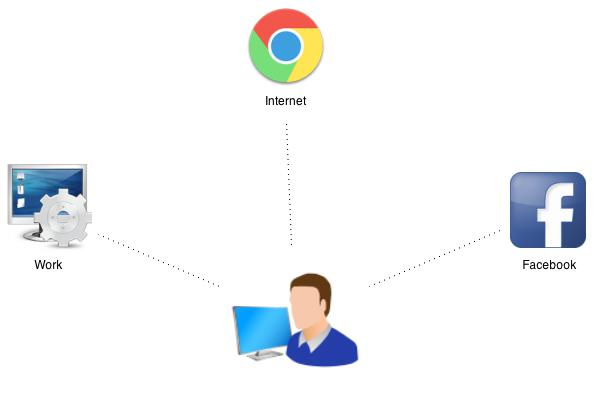
\includegraphics[scale=0.5]{Images/ambientesestudo.jpg}
   \caption{Ambientes de teste definidos}
\end{figure}

\section{Serviços Utilizados}

A decisão sobre os serviços de métrica a utilizar nestes testes esteve diretamente ligada aos sensores escolhidos e consequentemente ao tipo de dados recolhidos. Tal como já foi explicado a escolha dos sensores teve como um dos parâmetros a ter em conta a possibilidade de utilização de um grande número de métricas, pelo valor que estas acrescentam ao trabalho, mas também relativamente aos resultados que é possível obter.

Tendo por base estes aspetos, e tendo em conta que os sensores escolhidos foram sensores de rato, teclado e o acelerómetro, é possível utilizar todos os serviços de métricas integrados na arquitetura e apresentados no capítulo anterior. A utilização desta panóplia de serviços irá permitir alcançar um conjunto diversificado de indicadores, num nível de informação mais refinado e deste modo enriquecer os resultados desta demonstração.

\section{Resultados}

A experiência efetuada teve por base todas as decisões tomadas e explicadas neste capítulo. Isso permitiu definir um conjunto de pressupostos com o intuito de demonstrar a funcionalidade, interoperabilidade e utilidade da arquitetura desenvolvida, que é o seu principal objetivo. Pretende-se ainda apresentar diferenças percetíveis entre os resultados de monitorização dos utilizadores nos diversos momentos e ambientes definidos para este caso em particular. Desta forma serão apresentados os resultados alcançados, sublinhando determinados pontos e conclusões mais relevantes dado que o conjunto total de informação recolhido é bastante extenso.

Entre os diversos serviços de métricas integrados na arquitetura e utilizados nesta demonstração resultaram grandes blocos de informação cujos resultados se revelaram bastante úteis e esclarecedores em diversos aspetos. De forma a analisar os resultados alcançados serão apresentados nesta secção análises comparativas. Para cada análise serão selecionados resultados de três utilizadores da arquitetura. Os resultados apresentados foram selecionados por serem representativos da generalidade dos resultados alcançados, mas também por demonstrarem algumas características que se pretendia provar nesta experimentação.

Posto isto, e tal como já foi apresentado, estes testes foram feitos por um conjunto de utilizadores de forma a analisar os diferentes comportamentos em diversos parâmetros na execução de três tarefas diferentes. Uma dessas tarefas corresponde à utilização do Facebook. Neste aspeto o serviço de métricas que revelou resultados mais interessantes foi  o \textit{Writing Acceleration}. Este serviço de métrica, que corresponde aos dados recolhidos pelo sensor de teclado, apresenta a variação da velocidade de escrita por intervalo de tempo. A análise dos dados recolhidos e processados permite concluir que os três utilizadores escolhidos neste caso apresentaram resultados claramente distintos.


Estes resultados são bastante curiosos porque os três utilizadores tiveram um elevado número de registos de aceleração negativos, ou seja, perda de velocidade. Isto levou a que as médias apresentadas pelos três se situassem em bastante perto do valor zero. O primeiro utilizador foi o único que obteve uma média negativa, apesar de bastante perto do zero, e apresentou também o maior desvio padrão. O segundo utilizador teve a média mais elevada e o menor desvio padrão. Para além disso apresentou ainda os valores máximos e mínimos mais elevados para este caso em particular, como é possível também verificar pelo \textit{BoxPlot} apresentado. O terceiro utilizador obteve os resultados mais intermédios, de sublinhar apenas a sua mediana que apresentou valores negativos, ao contrário dos restantes utilizadores apresentados.

\begin{figure}[htb]
   \centering
   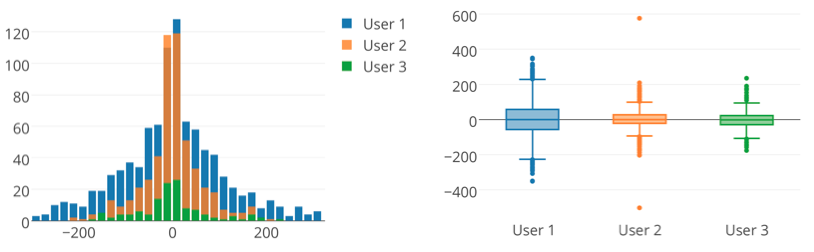
\includegraphics[scale=0.45]{Images/writingaccelerationfb.png}
   \caption{Histograma e BoxPlot de resultados de Writing Acceleration dos três utilizadores na utilização do Facebook}
\end{figure}

{\renewcommand{\arraystretch}{1.6}
\begin{table*}[!htb]
\centering
\label{tab:a_tbk}
\vspace{2pt}
\begin{tabular}{ | l | l | l | l | l | l |  }
\hline
\textit{Utilizador}&\textit{Média}&\textit{Desvio padrão}&\textit{Mediana} & \textit{Máximo} & \textit{Mínimo}\\  
\hline
1&-0.009719222&110.0210246&0&350&-351 \\
2&0.595419847&69.82373641&0&576&-502 \\
3&0.113821138&76.02352993&-2&235&-176 \\
\hline
\end{tabular}
\caption{Valores médios de Writing Acceleration dos três utilizadores na utilização do Facebook} 
\end{table*}}



A navegação de forma livre na Internet por parte dos utilizadores foi outro dos ambientes de monitorização ao qual estes foram sujeitos. No que diz respeito aos resultados obtidos através dos serviços de métricas importa realçar os resultados do \textit{Distance Between Clicks}. Esta métrica, referente aos dados provenientes da utilização do rato, representa a distância percorrida entre dois cliques consecutivos. Neste aspeto o segundo utilizador selecionado revelou-se o utilizador que menos distância percorre entre dois cliques, tal como indica a sua distância média. Como é possível verificar graficamente, grande parte dos registos do segundo utilizador centram-se em valores baixos, o que ajuda a explicar a sua distância média inferior aos restantes. O primeiro e terceiros utilizadores registam valores mais elevados para todos os parâmetros estatísticos apresentados, sendo o primeiro utilizador o detentor da média mais alta e o terceiro o que registo o valor máximo mais elevado. De salientar também que a diferença de médias do segundo para o primeiro utilizador já é uma diferença significativa.


\begin{figure}[htb]
   \centering
   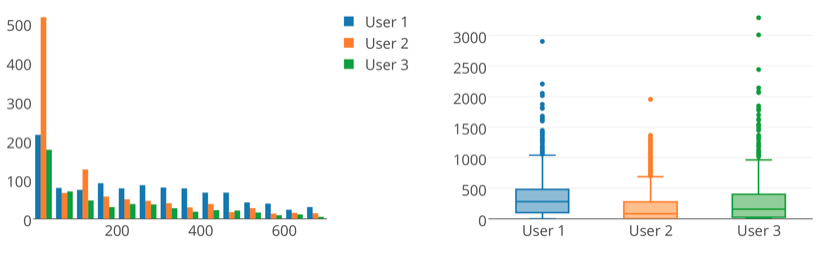
\includegraphics[scale=0.45]{Images/distancebetweenclicksnet.png}
   \caption{Histograma e BoxPlot de Distance Between Clicks dos três utilizadores na utilização da Internet}
\end{figure}

{\renewcommand{\arraystretch}{1.6}
\begin{table*}[!htb]
\centering
\label{tab:a_tbk}
\vspace{2pt}
\begin{tabular}{ | l | l | l | l | l | l |  }
\hline
\textit{Utilizador}&\textit{Média}&\textit{Desvio padrão}&\textit{Mediana} & \textit{Máximo} & \textit{Mínimo}\\  
\hline
1&347.7548827&336.7363147&278.8922&2902.985575&0 \\
2&187.637069&269.1631753&81.4272&1956.474051&0 \\
3&293.4572013&408.6060331&156.7983&3288.534389&0 \\
\hline
\end{tabular}
\caption{Valores médios de Distance Between Clicks dos três utilizadores na utilização da Internet} 
\end{table*}}


O outro contexto de monitorização definido foi o período de trabalho dos utilizadores. Este contexto normalmente é o mais intenso e desgastante dos três. De forma a poder comparar o desempenho neste ambiente são apresentados resultados de três utilizadores correspondentes à velocidade de escrita durante este período. 


 \begin{figure}[htb]
   \centering
   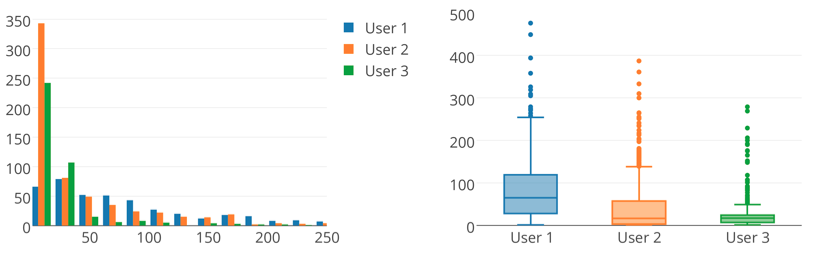
\includegraphics[scale=0.45]{Images/writingvelocitywork.png}
   \caption{Histograma e BoxPlot de Writing Velocity dos três utilizadores durante o período de trabalho}
\end{figure}

{\renewcommand{\arraystretch}{1.6}
\begin{table*}[!htb]
\centering
\label{tab:a_tbk}
\vspace{2pt}
\begin{tabular}{ | l | l | l | l | l | l |  }
\hline
\textit{Utilizador}&\textit{Média}&\textit{Desvio padrão}&\textit{Mediana} & \textit{Máximo} & \textit{Mínimo}\\  
\hline
1&87.93380615&84.94436633&65&476&1 \\
2&43.27126806&67.15051428&16&387&1 \\
3&25.25692695&37.8380318&17&279&1 \\
\hline
\end{tabular}
\caption{Valores médios de Writing Velocity dos três utilizadores durante o período de trabalho} 
\end{table*}}

Os resultados do terceiro utilizador demonstram que este foi o mais calmo, relativamente a a este aspeto, durante o seu período de trabalho, registando-se a maior parte dos seus registos nos valores mais baixos. O segundo utilizador teve resultados mais elevados que o terceiro, ainda assim verifica-se que, tal como o terceiro utilizador, a maior parte dos seus registos se encontram nos valores mais baixos. Por fim, o primeiro utilizador foi o que apresentou resultados mais elevados, o que indica maior intensidade no seu período de trabalho comparativamente com os restantes utilizadores. A média de resultados apresentada pelo primeiro utilizador é superior aos restantes, bem como o seu desvio padrão e mediana. 

Outra análise relevante que deve ser tida em conta é a comparação de resultados obtidos pelo mesmo utilizador na execução de diferentes tarefas. Esta comparação permitirá verificar a diferença de comportamento de um utilizador sob condições diferentes e retirar conclusões sobre esses factos. Posto isto, foram selecionados os resultados de um utilizador para a métrica de \textit{Absolute Sum of Angles} que permite quantificar o desvio do movimento do rato independentemente da sua direção. Os resultados desta métrica, teoricamente, terá tendência a apresentar valores mais altos em situações de maior desgaste ou stress, por exemplo.

Os resultados obtidos desta forma apresentam diferenças significativas entre a monitorização efetuada durante a utilização do Facebook e Internet em relação à monitorização durante o período de trabalho. Os valores obtidos durante os dois primeiros contextos apresentam valores bastante aproximados, tanto para os valores médios e desvios padrões como é, inclusivamente, visível graficamente. Esta semelhança de valores indica que em ambas as situações o utilizador teve comportamentos relativamente semelhantes neste parâmetro em particular. Já no que diz respeito ao período de trabalho as diferenças são bastante acentuadas. A média e desvio são bastante superiores, sendo até necessário utilizar uma escala bastante maior para apresentar o \textit{BoxPlot} dos resultados de monitorização do utilizador durante o período de trabalho . 

 \begin{figure}[htb]
   \centering
   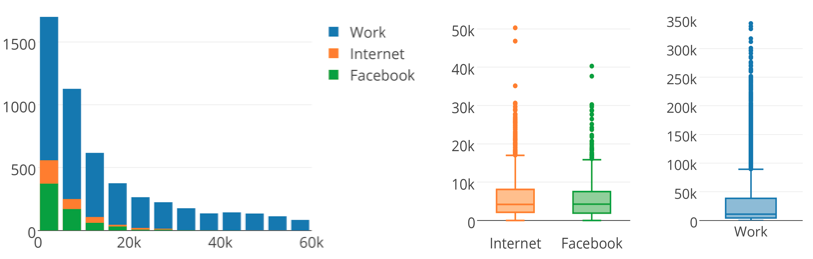
\includegraphics[scale=0.45]{Images/absolutesumofangles.png}
   \caption{Histograma e BoxPlot de Absolute Sum of Angles das três tarefas realizadas por um utilizador}
\end{figure}

{\renewcommand{\arraystretch}{1.6}
\begin{table*}[!htb]
\centering
\label{tab:a_tbk}
\vspace{2pt}
\begin{tabular}{ | l | l | l | l | l | l |  }
\hline
\textit{Tarefa}&\textit{Média}&\textit{Desvio padrão}&\textit{Mediana} & \textit{Máximo} & \textit{Mínimo}\\  
\hline
Trabalho&31452.38284&47164.0608&11005.6794&364649.1419&0 \\
Internet&6091.700595&5886.981361&4202.828&50268.26872&0 \\
Facebook&5855.7629&5633.691161&4285.8231&40281.81227&0 \\
\hline
\end{tabular}
\caption{Valores médios de Absolute Sum of Angles das três tarefas realizadas por um utilizador} 
\end{table*}}

Estes valores demonstram de facto uma diferença acentuada entre duas situações de lazer, navegar na Internet e utilização de Facebook, relativamente a uma situação de trabalho com toda a carga que este contexto implica. O facto de ser um contexto mais pesado e com maior probabilidade de existência de situações como a fadiga e stress, justifica a variação de resultados entre os contextos analisados neste caso particular.

A utilização do acelerómetro nesta experiência não foi tão profunda e abrangente como a dos restantes sensores. A sua utilização não foi orientada às três tarefas definidas mas apenas num contexto livre por dificuldade de acesso ao próprio dispositivo. Ainda assim, importa apresentar alguns resultados da sua utilização. Este tipo de dados também não tem, de momento, serviços de métricas desenvolvidos, contudo a análise dos seus resultados permite observar dados interessantes. Este tipo de sensor permitem verificar a aceleração ocorrida sobre três eixos, ou seja, permite obter a aceleração na diagonal, horizontal e vertical.

O acelerómetro foi utilizado sobre as pernas, rato, teclado e cadeiras dos seus utilizadores de forma a tentar abranger vários pontos corporais e de interação com o computador. Os resultados apresentados correspondem aos dados recolhidos sobre a aceleração de um utilizador sobre o seu movimento na cadeira. 

Como é possível verificar, os resultados indicam uma aceleração média positiva tanto na horizontal como na diagonal, ao contrário da aceleração verificada na vertical que indica que o movimento neste eixo tem uma variação média de velocidade negativa. De referir ainda que a aceleração na horizontal é a mais acentuada e a aceleração na diagonal contém alguns registos negativos.

 \begin{figure}[htb]
   \centering
   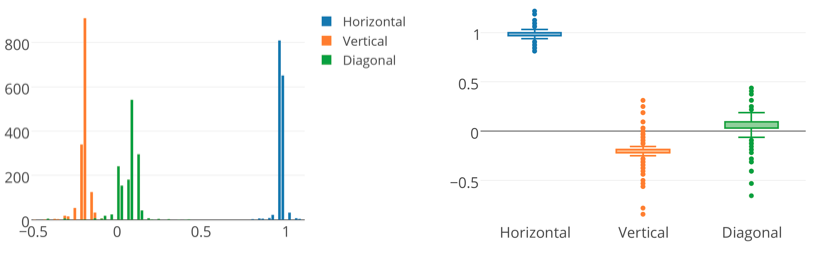
\includegraphics[scale=0.45]{Images/acceleration.png}
   \caption{Histograma e BoxPlot de resultados de acelerómetro sobre o movimento na cadeira}
\end{figure}

{\renewcommand{\arraystretch}{1.6}
\begin{table*}[!htb]
\centering
\label{tab:a_tbk}
\vspace{2pt}
\begin{tabular}{ | l | l | l | l | l | l |  }
\hline
\textit{Tarefa}&\textit{Média}&\textit{Desvio padrão}&\textit{Mediana} & \textit{Máximo} & \textit{Mínimo}\\  
\hline
Horizontal&0.98255158&0.025554207&0.9688&1.21875&0.8125 \\
Vertical&-0.192577369&0.053899455&-0.1875&0.3125&-0.84375 \\
Diagonal&0.067960187&0.074981723&0.0938&0.4375&-0.65625 \\
\hline
\end{tabular}
\caption{Valores médios de resultados de acelerómetro sobre o movimento na cadeira} 
\end{table*}}



\section{Conclusão/Sumario}

Esta experiência permitiu validar o funcionamento da arquitetura e dessa forma confirmar que a arquitetura desenvolvida é funcional e bastante útil para os seus utilizadores. Foi possível verificar que se trata de uma arquitetura com um funcionamento estável e cujas suas características e funcionalidades permitem uma recolha, tratamento e gestão da informação dos utilizadores fiáveis. A apresentação de diversos resultados e consequente análise do comportamento dos utilizadores efetuada neste capítulo demonstra que se trata de uma arquitetura com grande utilidade. A sua utilização em situações de monitorização, independentemente do contexto e localização dos dispositivos de recolha de informação, dá assim garantias de fiabilidade aos seus utilizadores.

Um fator importante para o sucesso desta demonstração foi o cuidado na escolha e definição de todos os parâmetros da experiência. A escolha de um conjunto heterogéneo de utilizadores, sob diferentes contextos de monitorização e ainda a seleção dos sensores a utilizar e consequentes serviços de métricas, confirmaram-se acertadas e contribuíram para a qualidade dos resultados. Para além disso, salientar ainda a demonstração de interoperabilidade da arquitetura. A utilização de sensores cujos \textit{gateways} são baseados em tecnologias diferentes atesta a capacidade dos métodos de comunicação implementados e de componentes com diferentes bases tecnológicas serem capazes de cooperar com sucesso.

Relativamente ao conteúdo dos resultados alcançados, estes foram bastantes satisfatórios. Para além de provarem a funcionalidade da arquitetura, permitiram verificar vários pontos e situações muito interessantes no que diz respeito ao comportamento dos utilizadores. De referir ainda que, num cômputo geral, os resultados alcançados foram de encontro ao que se pretendia na definição prévia de todas as características pensadas para esta experiência. Ou seja, todas as condições foram definidas de modo a que os resultados permitissem verificar algumas diferenças entre os contextos e resultados de cada utilizador. A análise final dos resultados confirmou a existência dessas diferenças tal como se pretendia.

A demonstração efetuada permitiu ainda verificar a utilidade dos serviços de métricas integrados na arquitetura. A utilização destes serviços na arquitetura permitiu analisar vários aspetos em particular e apresenta-los ao utilizador final, como estes resultados aqui apresentados demonstram. De assinalar ainda a diversidade de parâmetros e resultados obtidos através desta experiência. Apesar de apenas terem sido utilizados três tipos de sensores, para além das restantes condições definidas para este caso em particular, os resultados obtidos foram bastante abrangentes. Foi possível obter resultados de um número bastante alargado de aspetos e analisar o comportamento de cada utilizador nesses contextos.